\chapter{Simulazione}

Il progetto di tesi si propone di effettuare una simulazione, su base realistica, del funzionamento della blockchain utilizzata per i Bitcoin al fine di eseguire una analisi di alcune possibili attività malevole.\newline
Data la complessa struttura di una blockchain molte delle attività di ricerca in questo campo si sono focalizzate sulla formulazione teorica e matematica di questi scenari. L'obiettivo quindi è mettere in pratica diverse tipologie di attacco al fine di misurare fattibilità ed \textit{outcome} da parte di un avversario.\newlin\newline

La simulazione prevede l'esecuzione di scenari di attività malevole su struttura, rete e protocollo il più possibile attinenti alla realtà: propagazione dei messaggi, \textit{mining}, collaborazione tra nodi, raccolta delle transazioni. Questa necessità impone l'utilizzo di reti \textit{peer-to-peer} con un notevole numero di nodi, la possibilità di raccogliere dei dati a precisi timestamp e la possibilità di inserire alcuni scenari da applicare alla rete (\textit{forking attack}, \textit{Sybil attack}, \textit{51\%}).\newline
Innanzitutto è fondamentale ricostruire lo stack del protocollo Bitcoin eliminando quelle caratteristiche che lo rendono difficoltoso da simulare: mining, dimensione della blockchain, validazione delle transazioni, \textit{Merkle Tree}, decentralizzazione.\newline
Il mining deve essere una caratteristica controllata dall'analista in quanto è un fattore importante nell'analisi dei dati e, in aggiunta, non può rispecchiare tempistiche, dimensioni e difficoltà della rete attuale.\newline
Per quanto riguarda le transazioni e la decentralizzazione è necessario che la simulazione non interagisca con la reale rete di peer di Bitcoin ma che il tutto sia coordinato dal simulatore.\newline
Il primo problema fondamentale da risolvere è la simulazione di reti \textit{peer-2-peer} in quanto per loro natura sono non-strutturate e i collegamenti sono effettuati arbitrariamente e localmente. Un altro problema consiste nel progettare una struttura che utilizzi il protocollo di gossip per simulare l'interazione tra nodi Bitcoin senza però ricostruire l'intero stack del protocollo. L'obiettivo infatti è raggiungere una dimensione della rete \textit{p2p} che sia paragonabile a quella reale e che abbia comportamenti simili. La rete di simulazione deve essere sufficientemente grande da garantire che i risultati ottenuti siano spendibili e applicabili alla rete reale: un test eseguito su un numero ristretto di peer potrebbe portare ad analisi non corrette in quanto il fattore di randomizzazione della rete è applicato a meno peer\footnote{Con un campione ristretto esiste un maggior rischio che la rete \textit{p2p} sia completamente connessa e che i fattori come latenza, posizione nella rete possano rendere un attacco molto più (o meno) probabile.}.\newline
Il simulatore quindi deve essere altamente scalabile ed estensibile.\newline
Sono stati presi in considerazione diversi framework da utilizzare tra cui: \href{http://pads.cs.unibo.it/doku.php?id=pads:lunes}{\textit{LUNES}}, \href{https://www.nsnam.org/}{\textit{NS-3}} e una versione specializzata di \textit{NS-3}: \href{https://github.com/arthurgervais/Bitcoin-Simulator}{\textit{Bitcoin-Simulator}}. Il campo di scelta è ristretto a questi applicativi in quanto risultano essere testati ed usati in ambienti reali e/o accademici e altamente estensibili. I progetti sono open-source e quindi portabili su diverse architetture ed astraggono alcune funzionalità di base come la creazione della rete, dei collegamenti permettendo di lavorare solo sul core della simulazione.
\begin{figure}
    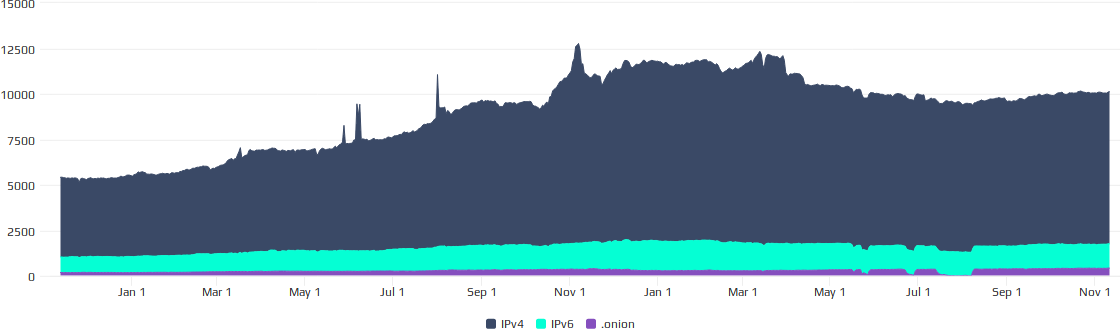
\includegraphics[width=\textwidth]{images/number_nodes.png}
    \caption{Numero di nodi rilevati negli ultimi due anni appartenenti alla rete Bitcoin (Novembre, 2018).}
    \source{bitnodes.earn.com}
\end{figure}

\section{\textit{NS-3}}
\textit{NS-3} è un simulatore di rete ad eventi discreti con licenza \textit{GNU GPLv2}. Lo scopo del progetto è di costruire di un solido nucleo di simulazione ben documentato, estensibile e che soddisfi le esigenze di un ciclo di vita di sviluppo del software.\newline
Il simulatore è stato progettato per supportare simulazioni su reti basate su protocollo IP ma grazie all'estensibilità è possibile modificarlo per l'utilizzo di altri protocolli di rete (ad esempio \href{https://named-data.net/}{\textit{NDN}}). Il core del simulatore si basa su uno schedulatore \textit{real-time} per la gestione dinamica degli eventi scatenati dai nodi che compongono la rete.\newline
Il codice può essere usato come libreria (sia statica che dinamica) con cui poter creare un progetto principale in \textit{C++} o \textit{Python} per definire la topologia della rete, il comportamento dei nodi, le interazioni e la raccolta dati. In aggiunta è possibile anche sviluppare delle interfacce grafiche tramite le apposite API per la visualizzazione dell'evoluzione della simulazione.
\begin{figure}[H]
    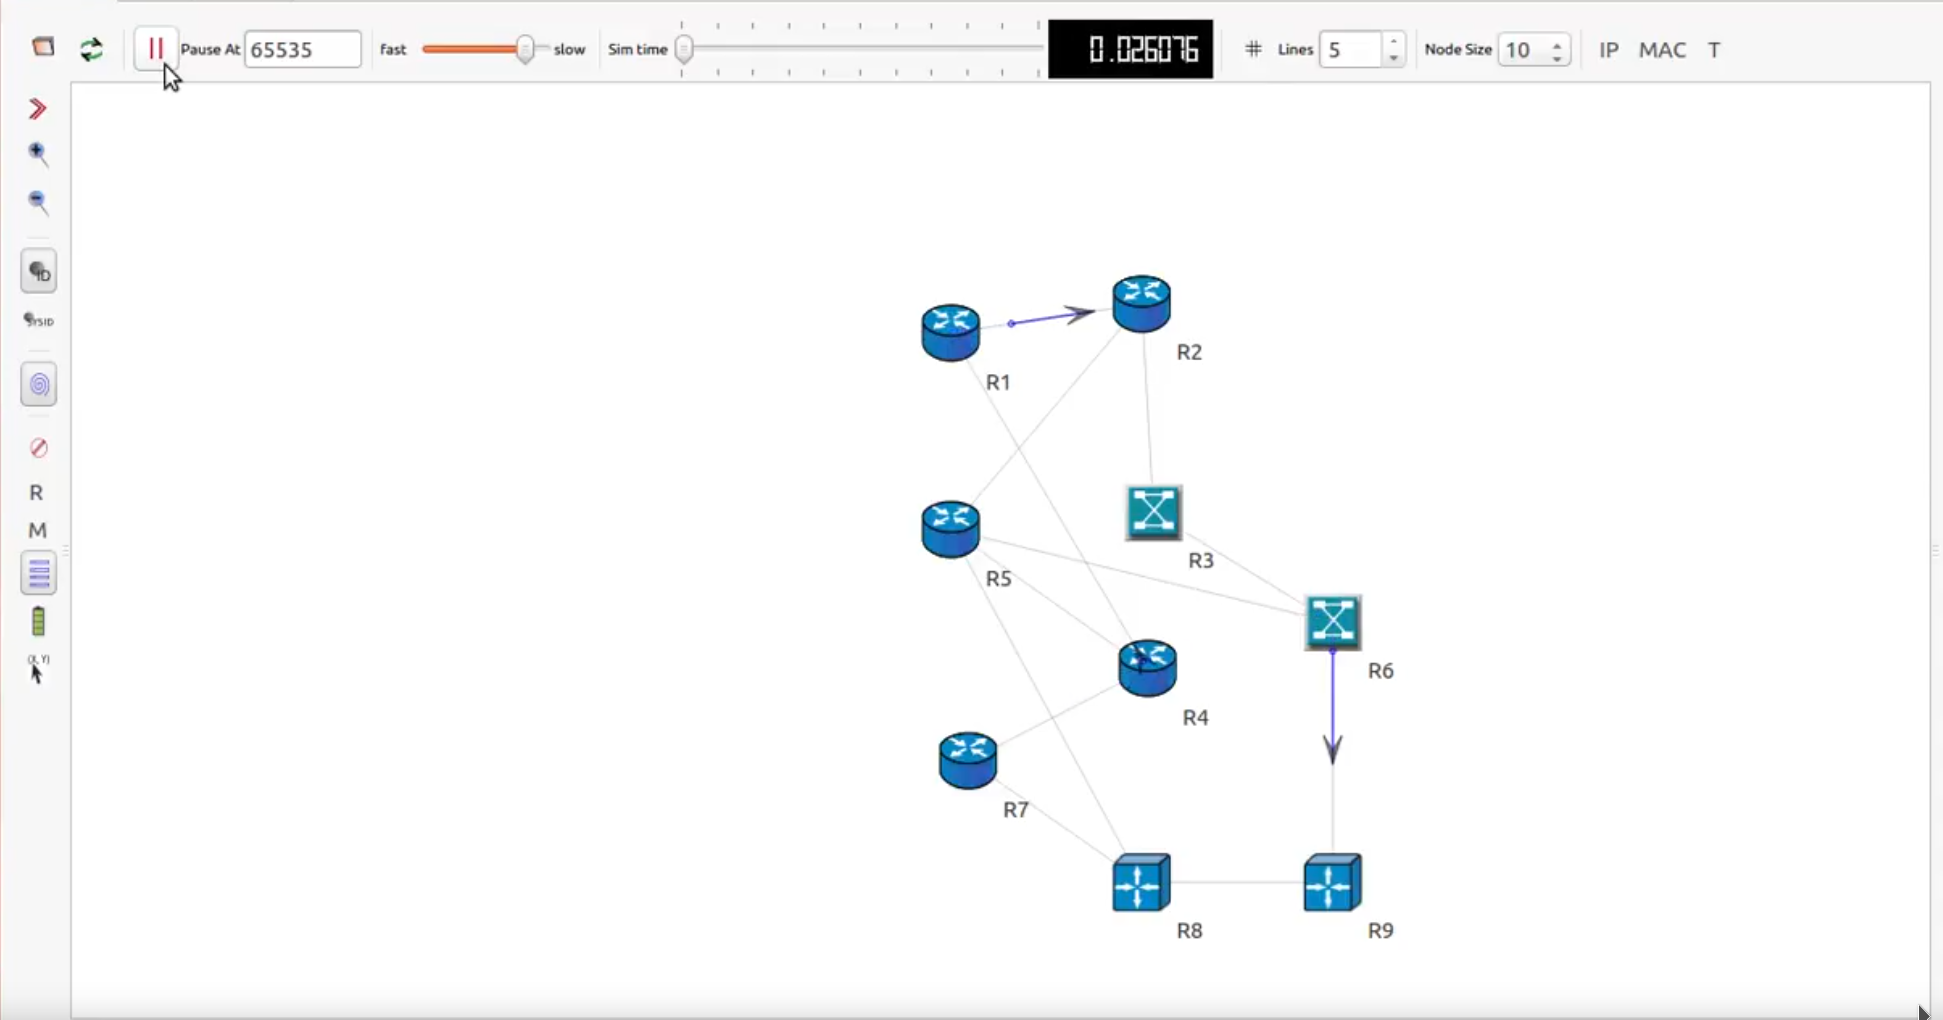
\includegraphics[width=\textwidth]{images/ns3.png}
    \caption{Esempio di simulazione con \textit{NS-3} per \textit{BGP}}
\end{figure}
Il simulatore, implementando dalla base l'intero stack di rete, permette una elevata personalizzazione e molteplici gradi di libertà nelle scelte progettuali: applicazioni, dispositivi di rete, modelli di movimento, modelli di propagazione, API per chiamate a primitive di basso livello. Ad esempio è possibile definire quale dispositivo di rete è utilizzato dai nodi (rete cablata o wireless), la latenza delle comunicazioni, la versione del protocollo (ad esempio \textit{802.11n} o \textit{802.11b}).\newline
Il caso preso in esame per la valutazione del simulatore \textit{NS-3} comprende le modifiche apportate da \textit{Arthur Gervais et al.} per uno studio sul consenso distribuito e come caratteristiche della rete e del protocollo affliggono la scalabilità e la sicurezza del \textit{POW} applicato alla blockchain Bitcoin.\newline
I risultati ottenuti dallo studio realizzato hanno portato osservazioni interessanti come l'impatto della dimensione del blocco, della latenza di rete, del numero di miner sia in condizioni normali che in condizioni di presenza di attori malevoli.
\begin{table}
    \centering
    \caption{Numero di blocchi \textit{stale} e transazioni per secondo raggiungibili con 16 miner nella rete e diverse dimensioni dei blocchi}
    \resizebox{\textwidth}{!}{\begin{tabular}{|c|c|c|c|}
        \hline
        \begin{tabular}[c]{@{}c@{}}Dimensione Blocco (MB)\end{tabular} &
        \begin{tabular}[c]{@{}c@{}}Intervallo (s)\end{tabular} &
        \begin{tabular}[c]{@{}c@{}}Blocchi \textit{stale} (s)\end{tabular} &
        \begin{tabular}[c]{@{}c@{}}Transazioni per secondo\end{tabular} \\\hline
        0.25 & 30 &	0.76 & 33.4  \\
        0.1  & 10 &	1.76 & 40    \\
        0.25 & 20 &	1.11 & 50    \\
        0.25 & 15 &	1.45 & 66.47 \\
        0.5  & 30 &	0.98 & 66.47 \\
        1    & 60 &	0.74 & 66.47 \\
        \hline
\end{tabular}}
\end{table}
In quanto il simulatore prende in considerazione tutti gli elementi dello stack di rete, l'esecuzione dei test risulta essere pesante e poco efficiente dal punto di vista di consumo delle risorse: un test con $10100$ nodi e circa $5000$ miner \footnote{Il numero è relativo alla reale rilevazione dei nodi conosciuti, il numero potrebbe essere superiore (fonte: \href{https://bitnodes.earn.com/nodes/}{https://bitnodes.earn.com/nodes/}).}, numeri realistici ed attuali, non è andato a buon fine su un device ad alte prestazioni.\newline
Tenendo conto della pesantezza e poca scalabilità del simulatore \textit{NS-3} per strutture molto estese e con poche esigenze di personalizzazione a basso livello si è deciso di trovare una alternativa. In aggiunta il codice utilizzato come estensione per la simulazione della Blockchain Bitcoin non è stato aggiornato dal 2016 e quindi non risulta essere compatibile con le nuove versioni del simulatore o cambiamenti ed evoluzione del protocollo.\newline
\begin{figure}
    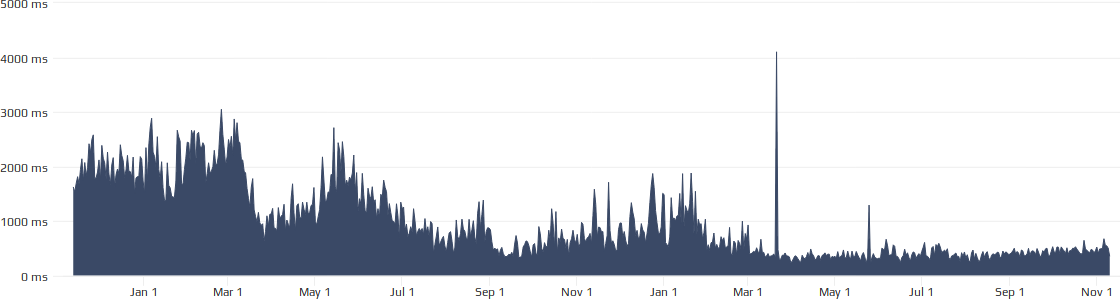
\includegraphics[width=\textwidth]{images/blocks_propagation.png}
    \caption{Propagazione dei blocchi negli ultimi due anni in \textit{millisecondi}, i dati sono stati campionati utilizzando i messaggi \texttt{inv} (messaggi inviati come aggiornamento su blocchi o transazioni tra i nodi, Novembre, 2018).}
    \source{bitnodes.earn.com}
\end{figure}

\section{\textit{LUNES}: Large Unstructured Network Simulator}
La completezza del simulatore \textit{NS-3} lo rende estremamente utile ma anche altamente complesso e poco performante in casi di reti molto grandi.\newline
Nonostante la superiorità del simulatore \textit{NS-3} questo non è stato scelto come base per il progetto di tesi in quanto, come descritto sopra, sono necessarie alcune caratteristiche fondamentali che il simulatore \textit{LUNES} rispetta.\newline
\textit{LUNES}\cite{gdalunes} è stato sviluppato da una gruppo di ricerca presso l'Università di Bologna, Dipartimento di Ingegneria e Scienze Informatiche (\textit{DISI}) per garantire il massimo dell'efficienza in simulazioni di protocollo complessi su reti in larga scala e non strutturata.\newline
Il simulatore si basa su una architettura distribuita e parallela basata su agenti e fornisce la possibilità di importare delle topologie di rete create anche con altri tool (e.g. \texttt{igraph}) ed astrae le complicazioni dovute alla gestione della rete \textit{p2p} implementando internamente i vari algoritmi di \textit{data dissemination}. \textit{LUNES} è stato progettato per dividere le operazioni di simulazione in tre fasi primarie:
\begin{enumerate}
    \item creazione della topologia di rete;
    \item simulazione del protocollo in uno specifico \textit{testbed};
    \item analisi dei risultati con i dati elaborati dal simulatore.
\end{enumerate}
La suddivisione in fasi permette anche al software di simulazione di essere modulare ed estensibile in quanto si basa sull'utilizzo di file di template. Le performance sono massimizzate grazie all'utilizzo del \textit{middleware} \texttt{ARTÌS} e del \textit{framework} \texttt{GAIA}; i due strumenti sono stati sviluppato secondo l'approccio \textit{Parallel and Distribute Simulation} (\textit{PADS}) che fornisce un buon grado di scalabilità. \textit{LUNES}, infatti, utilizza delle API ad alto livello fornite dal framework GAIA.
\textit{LUNES} permette un approccio \texttt{time-step} per la simulazione: semplifica il deploy su architetture parallele e distribuite e permette di implementare delle tecniche di bilanciamento del carico per il middleware \texttt{ARTÌS}.
La simulazione è \textit{time-step} in quanto il tempo viene suddiviso in fasi sequenziali di una certa durata: l'avanzare degli step di simulazione non permette che il vincolo di casualità sia mai violato. La divisione in \textit{time-step} permette di avere un visione discreta degli eventi e poter controllare il tempo: sapendo quanto tempo impiega un evento è possibile evitare di aspettare prima che si verifichi.
\begin{table}[H]
    \resizebox{\textwidth}{!}{\begin{tabular}{|l|c|c|c|c|}
        \hline
        \begin{tabular}[c]{@{}c@{}}Algoritmo\end{tabular} &
        \begin{tabular}[c]{@{}c@{}}$100\%$\end{tabular} &
        \begin{tabular}[c]{@{}c@{}}$99\%$\end{tabular} &
        \begin{tabular}[c]{@{}c@{}}$90\%$\end{tabular} &
        \begin{tabular}[c]{@{}c@{}}$75\%$\end{tabular} &
        \hline
        Probabilità Fissa               & 3.00 (4.65) & 2.74 (4.86) & 1.80 (6.10) & 1.20 (7.62)\\
        Probabilistico                  & 3.00 (4.65) & 2.84 (4.76) & 2.03 (5.54) & 1.38 (6.49)\\
        Dipendente dal grado $\gamma_1$ & 2.99 (4.66) & 2.24 (5.59) & 1.48 (7.72) & 1.06 (9.11)\\
        Dipendente dal grado $\gamma_2$ & 2.99 (4.67) & 2.16 (5.88) & 1.48 (7.74) & 1.07 (8.99)\\
        \hline
    \end{tabular}}
    \caption{Overhead (e ritardo) di copertura per ciascun algoritmo per una rete di $500$ nodi, $1000$ archi, diametro to $10$, \texttt{TTL}$=16$ e cache fissa a $256$ simulata tramite \textit{LUNES}}
    \source{Highly intensive data dissemination in complex networks \cite{gdalunes}}
\end{table}
La comunicazione avviene tramite un insieme di \textit{Logical Process} (\texttt{LP}) che interagiscono tramite primitive di comunicazione: ogni thread è dedicato alla gestione della comunicazione su un singolo canale di input o output. Ogni \texttt{LP} costituisce una unità di esecuzione: il middleware permette di non dover gestire le unità di esecuzione come processi locali, remoti e la loro interazione. Ogni unità ha lo scopo di far progredire la simulazione comunicando con gli altri \texttt{LP}. Ogni \texttt{LP}, al fine di garantire il massimo della scalabilità, esegue diverse \textit{Simulated Entities} (\texttt{SE}); queste unità sono allocate dinamicamente e costituiscono la minima suddivisione del modello.\newline
Ogni \texttt{LP} viene eseguito da diversi \textit{Physical Execution Units} (\texttt{PEU}) che forniscono il livello di comunicazione tramite memoria condivisa o protocollo di rete.
\begin{figure}[H]
    \centering
    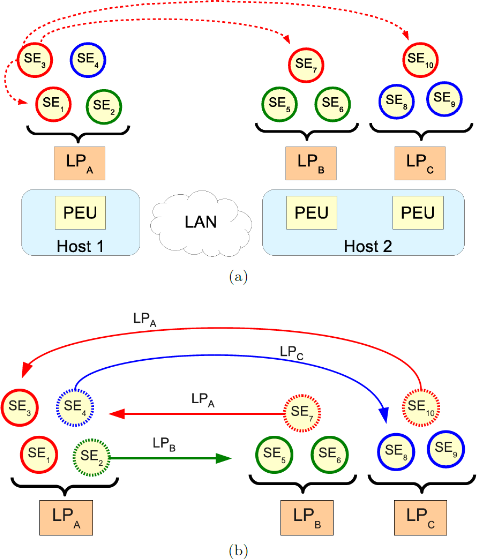
\includegraphics[width=0.7\textwidth]{images/PADS_example.png}
    \caption{Esempio di configurazione di un sistema \texttt{PADS}}
    \source{Design, implementation and performance evaluation of an anonymous distributed simulator \cite{antonio}}
\end{figure}
Un esempio di utilizzo di \textit{LUNES} per topologie di grandi dimensioni ad alte performance è dato da: un insieme di peer wireless si muovono in campo toroidale 2D; la loro interazione avviene per prossimità ed in broadcast. Il codice di esempio viene fornito assieme ai sorgenti del simulatore ed è utilizzato come base per utilizzi più avanzati.\newline
Il simulatore crea un numero di peer wireless che possono muoversi in uno spazio 2D toroidale secondo il modello \textit{Random Way Point}. Ogni nodo creato ha un raggio di azione massimo con cui può interagire con gli altri peer immersi nello spazio: quando $a$ è nel raggio di azione di $b$ allora verrà registrato l'invio di un messaggio da $b$ ad $a$. In questo caso viene inviato un messaggio di \texttt{ping}. I dati in output proposti dal simulatore sono personalizzabili nel codice della simulazione stessa grazie a delle API che permettono di tener traccia sia dei tempi di esecuzione (ad esempio gli \texttt{step} della simulazione), il tempo totale di esecuzione o le interazioni).
Tramite l'output fornito dalla simulazione è quindi possibile verificare, per ogni istante di tempo simulato, i vari stati dei nodi.
\begin{figure}[H]
    \centering
    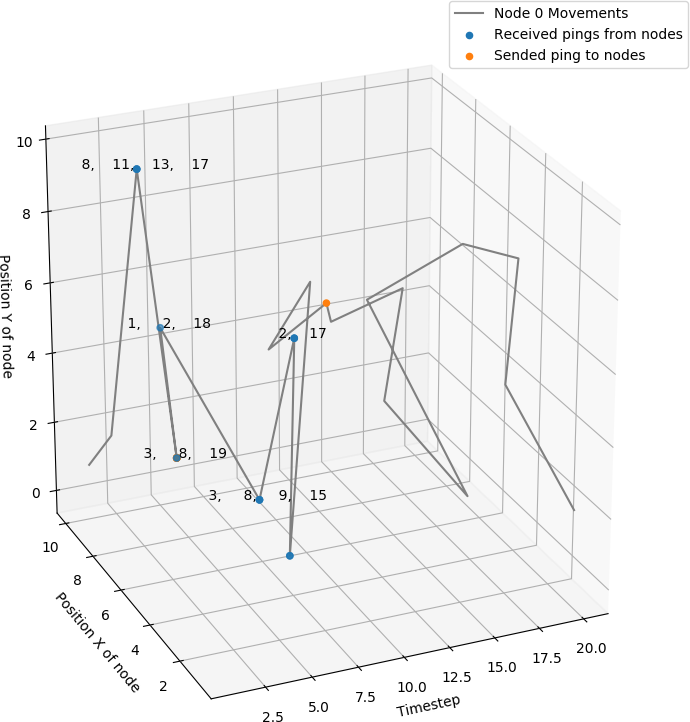
\includegraphics[width=0.9\textwidth]{images/lunes_wireless_plot.png}
    \caption{Visualizzazione dei movimenti di un nodo, i punti in cui ci sono state delle interazioni e i nomi dei nodi che hanno inviato dei \texttt{ping}}
\end{figure}
In termini di performance il simulatore risulta essere molto competitivo: lo stesso esempio, eseguito con una configurazione di $1$ \texttt{LP} e $20000$ peer, ha prodotto i seguenti risultati:
\begin{itemize}
    \item Tempo di esecuzione: $645.03s$
    \item Percentuale di copertura: $100.0$
    \item Numero totale di \texttt{ping} inviati: $194341876$
    \item Numero totale di \texttt{ping} ricevuti: $194341876$
\end{itemize}
Raddoppiando il numero di $LP$ disponibili il tempo di esecuzione è stato ridotto del $12.4\%$.

\subsection{ARTÌS: \textit{Advanced RTI System}}
\texttt{ARTÌS}\cite{artis} è un middleware adattivo fortemente basato sul riutilizzo delle componenti, orientato alla simulazione parallela e distribuita. Fornisce i meccanismi di gestione delle comunicazioni tra gli \texttt{LP}.\newline
In quanto i runtime possono risultare poco trasparenti all'utente finale durante l'esecuzione, è stato previsto un meccanismo di introspezione attraverso il quale gran parte delle informazioni interne sono rese disponibili tramite la modalità di \textit{publish/subscribe}.\newline
\texttt{ARTÌS} utilizza le API del il \textit{Simulation Manager} (\texttt{SIMA}) per l'inizializzazione e terminazione della simulazione la gestione le barriere di sincronizzazione e la coordinazione tra i vari \texttt{LP}. L'utilizzo del \textit{Simulation Manager} rende quindi l'architettura parzialmente decentralizzata.
\begin{itemize}
    \item \texttt{void SIMA Initialize(porta, lps, channel.txt)}: indica al \texttt{SIMA} quanti \texttt{LP} sono presenti, quale porta è utilizzata per le comunicazioni e da quale file leggere le configurazioni dei canali di comunicazione:
        \begin{itemize}
            \item[] \begin{lstlisting}[caption={Esempio di configurazione}]
            # DEFINIZIONE DEI CANALI:
            :MILANO 0
            :BOLOGNA 1
            :ROMA 2
            #DEFINIZIONE DEI LOOKAHEAD
            GLOBAL LA=0 # Look−Ahead Globale Disabilitato
            MILANO: BOLOGNA 5 ROMA 7
            ROMA: MILANO 7 BOLOGNA 3
            BOLOGNA: MILANO 5 ROMA 3
            \end{lstlisting}
        \end{itemize}
    \item \texttt{void SIMA Finalize()}: chiude la comunicazione tra \texttt{SIMA} e \texttt{LP} e le risorse allocate in fase di inizializzazione sono rilasciate;
    \item \texttt{void SIMA Barrier()}: istituisce un punto di sincronizzazione.
\end{itemize}

\subsection{GAIA: \textit{Generic Adaptive Interaction Architecture}}
\texttt{GAIA}\cite{padssite} è un framework l'ottimizzazione dell'esecuzione della simulazione. Il framework di riutilizzare le entità riducendo i tempi di esecuzione e l'overhead generato dalle comunicazioni sviluppate utilizzando \texttt{ARTÌS}.\newline
Una serie di euristiche valutano il pattern di comunicazione ed eventualmente schedulano una riallocazione degli oggetti.
Il framework supporta il paradigma  multiagente \texttt{MAS} (\textit{multi-agent system}) e la possibilità di eseguire su cluster eterogenei.
Un sistema multiagente è un sistema composto da molteplici agenti che interagiscono tra loro; questo approccio permette che ogni singolo agente sia autonomo, che abbia solo una visione locale e che il sistema complessivamente sia decentralizzato. Una delle più diffuse applicazioni per questi sistemi è l'utilizzo in tecnologie mobili e di rete per garantire un bilanciamento del carico automatico e dinamico, alta scalabilità e fault tollerance.

% NeoTex: mainfile=main.tex:
